% Copyright (C) 2014-2020 by Thomas Auzinger <thomas@auzinger.name>

\documentclass[draft,final]{vutinfth} % Remove option 'final' to obtain debug information.

% Load packages to allow in- and output of non-ASCII characters.
\usepackage{lmodern}        % Use an extension of the original Computer Modern font to minimize the use of bitmapped letters.
\usepackage[T1]{fontenc}    % Determines font encoding of the output. Font packages have to be included before this line.
\usepackage[utf8]{inputenc} % Determines encoding of the input. All input files have to use UTF8 encoding.

% Extended LaTeX functionality is enables by including packages with \usepackage{...}.
\usepackage{amsmath}    % Extended typesetting of mathematical expression.
\usepackage{amssymb}    % Provides a multitude of mathematical symbols.
\usepackage{mathtools}  % Further extensions of mathematical typesetting.
\usepackage{microtype}  % Small-scale typographic enhancements.
\usepackage[inline]{enumitem} % User control over the layout of lists (itemize, enumerate, description).
\usepackage{multirow}   % Allows table elements to span several rows.
\usepackage{booktabs}   % Improves the typesettings of tables.
\usepackage{subcaption} % Allows the use of subfigures and enables their referencing.
\usepackage[ruled,linesnumbered,algochapter]{algorithm2e} % Enables the writing of pseudo code.
\usepackage[usenames,dvipsnames,table]{xcolor} % Allows the definition and use of colors. This package has to be included before tikz.
\usepackage{nag}       % Issues warnings when best practices in writing LaTeX documents are violated.
\usepackage{todonotes} % Provides tooltip-like todo notes.
\usepackage[backend=biber,style=trad-alpha,isbn=false,eprint=false,maxcitenames=3]{biblatex}
\usepackage{hyperref}  % Enables cross linking in the electronic document version. This package has to be included second to last.
\usepackage[acronym,toc]{glossaries} % Enables the generation of glossaries and lists fo acronyms. This package has to be included last.
\usepackage{siunitx}
\usepackage{float}

\addbibresource{references.bib}

% Define convenience functions to use the author name and the thesis title in the PDF document properties.
\newcommand{\authorname}{Tobias Eidelpes} % The author name without titles.
\newcommand{\thesistitle}{Plant Detection and State Classification with Machine Learning} % The title of the thesis. The English version should be used, if it exists.

% Set PDF document properties
\hypersetup
{
    pdfpagelayout   = TwoPageRight,           % How the document is shown in PDF viewers (optional).
    linkbordercolor = {Melon},                % The color of the borders of boxes around crosslinks (optional).
    pdfauthor       = {\authorname},          % The author's name in the document properties (optional).
    pdftitle        = {\thesistitle},         % The document's title in the document properties (optional).
    pdfsubject      = {Subject},              % The document's subject in the document properties (optional).
    pdfkeywords     = {Object Detection, Image Classification, Machine Learning, Embedded Programming} % The document's keywords in the document properties (optional).
}

\setpnumwidth{2.5em}        % Avoid overfull hboxes in the table of contents (see memoir manual).
\setsecnumdepth{subsection} % Enumerate subsections.

\nonzeroparskip             % Create space between paragraphs (optional).
\setlength{\parindent}{0pt} % Remove paragraph identation (optional).

\setcounter{tocdepth}{3}

\makeindex      % Use an optional index.
\makeglossaries % Use an optional glossary.
%\glstocfalse   % Remove the glossaries from the table of contents.

% Set persons with 4 arguments:
%  {title before name}{name}{title after name}{gender}
%  where both titles are optional (i.e. can be given as empty brackets {}).
\setauthor{}{\authorname}{BSc}{male}
\setadvisor{Ao.Univ.-Prof. Dr.}{Horst Eidenberger}{}{male}

\setregnumber{01527193}
\setdate{20}{02}{2023} % Set date with 3 arguments: {day}{month}{year}.
\settitle{\thesistitle}{Plant Detection and State Classification with Machine Learning} % Sets English and German version of the title (both can be English or German).

% Select the thesis type: bachelor / master / doctor / phd-school.
% Master:
\setthesis{master}
\setmasterdegree{dipl.} % dipl. / rer.nat. / rer.soc.oec. / master

% For bachelor and master:
\setcurriculum{Software Engineering \& Internet Computing}{Software Engineering \& Internet Computing} % Sets the English and German name of the curriculum.

\newacronym{xai}{XAI}{Explainable Artificial Intelligence}
\newacronym{grad-cam}{Grad-CAM}{Gradient-weighted Class Activation Mapping}
\newacronym{cam}{CAM}{Class Activation Mapping}
\newacronym{oid}{OID}{Open Images Dataset}
\newacronym{ap}{AP}{Average Precision}
\newacronym{iou}{IOU}{Intersection over Union}
\newacronym{map}{mAP}{mean average precision}
\newacronym{resnet}{ResNet}{Residual Neural Network}
\newacronym{cnn}{CNN}{Convolutional Neural Network}
\newacronym{sgd}{SGD}{Stochastic Gradient Descent}
\newacronym{roc}{ROC}{Receiver Operating Characteristic}
\newacronym{auc}{AUC}{Area Under the Curve}

\begin{document}

\frontmatter % Switches to roman numbering.
% The structure of the thesis has to conform to the guidelines at
%  https://informatics.tuwien.ac.at/study-services

\addtitlepage{naustrian} % German title page (not for dissertations at the PhD School).
\addtitlepage{english} % English title page.
\addstatementpage

\begin{danksagung*}
\todo{Ihr Text hier.}
\end{danksagung*}

\begin{acknowledgements*}
\todo{Enter your text here.}
\end{acknowledgements*}

\begin{kurzfassung}
\todo{Ihr Text hier.}
\end{kurzfassung}

\begin{abstract}
\todo{Enter your text here.}
\end{abstract}

% Select the language of the thesis, e.g., english or naustrian.
\selectlanguage{english}

% Add a table of contents (toc).
\tableofcontents % Starred version, i.e., \tableofcontents*, removes the self-entry.

% Switch to arabic numbering and start the enumeration of chapters in the table of content.
\mainmatter

\chapter{Introduction}
\label{chap:introduction}

Machine learning has seen an unprecedented rise in various research
fields during the last few years. Large-scale distributed computing
and advances in hardware manufacturing have allowed machine learning
models to become more sophisticated and complex. Multi-billion
parameter deep learning models show best-in-class performance in
Natural Language Processing (NLP)~\cite{brown2020}, fast object
detection~\cite{bochkovskiy2020} and various classification
tasks~\cite{zhong2022,ariss2022}. Agriculture is one of the areas
which profits substantially from the automation possible with machine
learning.

Large-scale as well as small local farmers are able to survey their
fields and gardens with drones or stationary cameras to determine soil
and plant condition as well as when to water or
fertilize~\cite{ramos-giraldo2020}. Machine learning models play an
important role in that process because they allow automated
decision-making in real time.

\section{Motivation and Problem Statement}
\label{sec:motivation}

The challenges to implement an automated system are numerous. First,
gathering data in the field requires a network of sensors which are
linked to a central server for processing. Since communication between
sensors is difficult without proper infrastructure, there is a high
demand for processing the data on the sensor
itself~\cite{mcenroe2022}. Second, differences in local soil, plant
and weather conditions require models to be optimized for these
diverse inputs. Centrally trained models often lose the nuances
present in the data because they have to provide actionable
information for a larger area~\cite{awad2019}. Third, specialized
methods such as hyper- or multispectral imaging in the field provide
fine-grained information about the object of interest but come with
substantial upfront costs.

To address all of the aforementioned problems, there is a need for an
installation which is deployable in the field, gathers data using
readily available hardware and performs computation on the device
without a connection to a central server. The device should be able to
visually determine whether the plants in its field of view need water
or not and output its recommendation.

The aim of this work is to develop a prototype which can be deployed
in the field to survey plants and recommend watering or not. To this
end, a machine learning model will be trained to first identify the
plants in the field of view and then to determine if the plants need
water or not. The model should be suitable for edge devices equipped
with a TPU or GPU but with otherwise limited processing
capabilities. Examples of such systems include Google's Coral
development board and the Nvidia Jetson series of single-board
computers (SBCs). The model should make use of state-of-the-art
algorithms from either classical machine learning or deep
learning. The literature review will yield an appropriate machine
learning method. Furthermore, the adaption of existing models
(transfer learning) for object detection to the domain of plant
recognition may provide higher performance than would otherwise be
achievable within the time constraints.

The model will be deployed to the single-board computer and evaluated
in the field. The evaluation will seek to answer the following
questions:

\begin{enumerate}
\item \emph{How well does the model work in theory and how well in
    practice?}

  We will measure the performance of our model with
  common metrics such as accuracy, F-score, receiver operating
  characteristics (ROC) curve, and area under curve (AUC). These
  measurements will allow comparisons between our model and existing
  models. We expect the plant detection part of the model to achieve
  high scores on the test dataset. However, the classification of
  plants into stressed and non-stressed will likely prove to be more
  difficult. The model is limited to physiological markers of water
  stress and thus will have difficulties with plants which do not
  overtly display such features.

  Even though models may work well in theory, some do not easily
  transfer to practical applications. It is, therefore, important to
  examine if the model is suited for productive use in the field. The
  evaluation will contain a discussion about the model's
  transferability because theoretical performance does not
  automatically guarantee real-world performance due to different
  environmental conditions.
\item \emph{What are possible reasons for it to work/not work?}

  Even if a model scores high on performance metrics, there might be a
  mismatch between how researchers think it achieves its goal and how
  it actually achieves its goal. The results have to be plausible and
  explainable with its inputs. Otherwise, there can be no confidence
  in the model's outputs. Conversely, if the model does not work,
  there must be a reason. We estimate that the curation of the dataset
  for the training and test phases will play a significant
  role. Explanations for model out- or underperformance are likely to
  be found in the structure and composition of the model's inputs.
\item \emph{What are possible improvements to the system in the
    future?}

  The previous two questions will yield the data for possible
  improvements to the model and/or our approach. With the decision to
  include a plant detection step at the start, we hope to create
  consistent conditions for the stress classification. A downside to
  this approach is that errors during detection can be propagated
  through the system and result in adverse effects to overall
  performance. Although we estimate this problem to be negligible,
  additional feedback regarding our approach in this way might offer
  insight into potential improvements. If the model does not work as
  well as expected, which changes to the approach will yield a better
  result? Similarly to the previous question, the answer will likely
  lie in the dataset. A heavy focus on dataset construction and
  curation will ensure satisfactory model performance.
\end{enumerate}

\section{Methodological Approach}
\label{sec:methods}

The methodological approach consists of the following steps and is
also shown in Figure~\ref{fig:setup}:

\begin{description}
\item[Literature Review] The literature review informs the type of
  machine learning methods which are later applied during the
  implementation of the prototype.
\item[Object Detection] Flowers present in the image will be detected
  using object detection methods. These methods will draw bounding
  boxes around the objects of interest. The output is fed into the
  next stage.
\item[State Classification] The bounded images will be fed to a
  classifier which will determine whether the plant needs water or
  not.
\item[Deployment to SBC] The software prototype will be deployed to
  the single-board computer in the field.
\item[Evaluation] The prototype will be evaluated in the field to
  determine its feasibility and performance. During evaluation the
  author seeks to provide a basis for answering the research
  questions.
\end{description}

\begin{figure}{H}
  \centering
  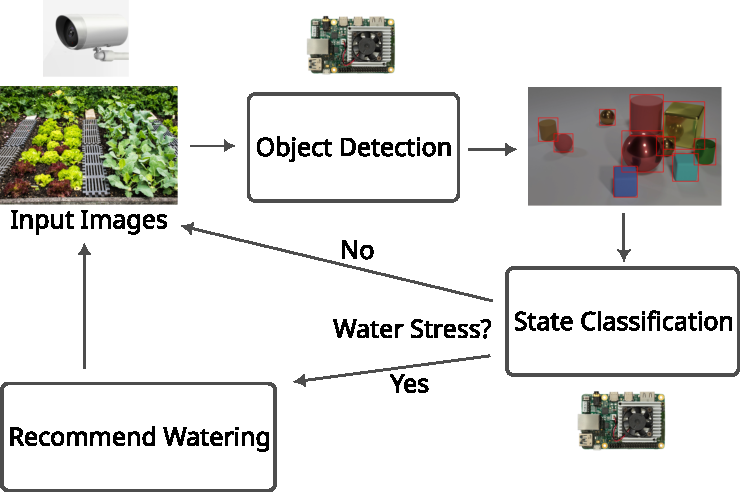
\includegraphics[width=0.8\textwidth]{graphics/setup.pdf}
  \caption{Setup in the field for water stress classification.}
  \label{fig:setup}
\end{figure}

\section{Thesis Structure}
\label{sec:structure}

The first part of the thesis contains the theoretical basis of the
models which we use for the prototype. 

\chapter{Theoretical Background}
\label{chap:background}

Describe the contents of this chapter.

\begin{itemize}
\item Related Work. (3 pages)
\item Description of inner workings of YOLOv7 as the object detection
  model. (4 pages)
\item Description of inner workings of ResNet as the classification
  model. (2 pages)
\end{itemize}

Estimated 9 pages for this chapter.

\section{Related Work}
\label{sec:related-work}

The literature on machine learning in agriculture is broadly divided
into four main areas:~livestock management, soil management, water
management, and crop management~\cite{benos2021}. Of those four, water
management only makes up about 10\% of all surveyed papers during the
years 2018--2020. This highlights the potential for research in this
area to have a high real-world impact.

\textcite{su2020} used traditional feature extraction and
pre-processing techniques to train various machine learning models for
classifying water stress for a wheat field. They took top-down images
of the field using an unmanned aerial vehicle (UAV), segmented wheat
pixels from background pixels and constructed features based on
spectral intensities and color indices. The features are fed into a
support vector machine (SVM) with a Gaussian kernel and optimized
using Bayesian optimization. Their results of 92.8\% accuracy show
that classical machine learning approaches can offer high
classification scores if meaningful features are chosen. One
disadvantage is that feature extraction is often a tedious task
involving trial and error. Advantages are the small dataset and the
short training time ($\qty{3}{\second}$) required to obtain a good
result.

Similarly, \textcite{lopez-garcia2022} investigated the potential for
UAVs to determine water stress for vineyards using RGB and
multispectral imaging. The measurements of the UAV were taken at
$\qty{80}{\meter}$ with a common off-the-shelf APS-C sensor. At the
same time, stem water measurements were taken with a pressure chamber
to be able to evaluate the performance of an artificial neural network
(ANN) against the ground truth. The RGB images were used to calculate
the green canopy cover (GCC) which was also fed to the model as
input. The model achieves a high determination coefficient $R^{2}$ of
$0.98$ for the 2018 season on RGB data with a relative error of
$RE = \qty{10.84}{\percent}$. However, their results do not transfer
well to the other seasons under survey (2019 and 2020).

\textcite{zhuang2017} showed that water stress in maize can be
detected early on and, therefore, still provide actionable information
before the plants succumb to drought. They installed a camera which
took $640\times480$ pixel RGB images every two hours. A simple linear
classifier (SVM) segmented the image into foreground and background
using the green color channel. The authors constructed a
fourteen-dimensional feature space consisting of color and texture
features. A gradient boosted decision tree (GBDT) model classified the
images into water stressed and non-stressed and achieved an accuracy
of $\qty{90.39}{\percent}$. Remarkably, the classification was not
significantly impacted by illumination changes throughout the day.

\textcite{an2019} used the ResNet50 model as a basis for transfer
learning and achieved high classification scores (ca. 95\%) on
maize. Their model was fed with $640\times480$ pixel images of maize
from three different viewpoints and across three different growth
phases. The images were converted to grayscale which turned out to
slightly lower classification accuracy. Their results also highlight
the superiority of deep convolutional neural networks (DCNNs) compared
to manual feature extraction and gradient boosted decision trees
(GBDTs).

\textcite{chandel2021} investigated deep learning models in depth by
comparing three well-known CNNs. The models under scrutiny were
AlexNet, GoogLeNet, and Inception V3. Each model was trained with a
dataset containing images of maize, okra, and soybean at different
stages of growth and under stress and no stress. The researchers did
not include an object detection step before image classification and
compiled a fairly small dataset of 1200 images. Of the three models,
GoogLeNet beat the other two with a sizable lead at a classification
accuracy of >94\% for all three types of crop. The authors attribute
its success to its inherently deeper structure and application of
multiple convolutional layers at different stages. Unfortunately, all
of the images were taken at the same $\ang{45}\pm\ang{5}$ angle and it
stands to reason that the models would perform significantly worse on
images taken under different conditions.

\textcite{ramos-giraldo2020} detected water stress in soybean and corn
crops with a pretrained model based on DenseNet-121. Low-cost cameras
deployed in the field provided the training data over a 70-day
period. They achieved a classification accuracy for the degree of
wilting of 88\%.

In a later study, the same authors~\cite{ramos-giraldo2020a} deployed
their machine learning model in the field to test it for production
use. They installed multiple Raspberry Pis with attached Raspberry Pi
Cameras which took images in $\qty{30}{\minute}$ intervals. The
authors had difficulties with cameras not working and power supply
issues. Furthermore, running the model on the resource-constrained
RPis proved difficult and they had to port their TensorFlow model to a
TensorFlow Lite model. This conversion lowered their classification
scores slightly since it was sometimes off by one water stress
level. Nevertheless, their architecture allowed for reasonably high
classification scores on corn and soybean with a low-cost setup.

\textcite{azimi2020} demonstrate the efficacy of deep learning models
versus classical machine learning models on chickpea plants. The
authors created their own dataset in a laboratory setting for stressed
and non-stressed plants. They acquired 8000 images at eight different
angles in total. For the classical machine learning models, they
extracted feature vectors using scale-invariant feature transform
(SIFT) and histogram of oriented gradients (HOG). The features are fed
into three classical machine learning models: support vector machine
(SVM), k-nearest neighbors (KNN), and a decision tree (DT) using the
classification and regression (CART) algorithm. On the deep learning
side, they used their own CNN architecture and the pre-trained
ResNet-18 model. The accuracy scores for the classical models was in
the range of $\qty{60}{\percent}$ to $\qty{73}{\percent}$ with the SVM
outperforming the two others. The CNN achieved higher scores at
$\qty{72}{\percent}$ to $\qty{78}{\percent}$ and ResNet-18 achieved
the highest scores at $\qty{82}{\percent}$ to
$\qty{86}{\percent}$. The results clearly show the superiority of deep
learning over classical machine learning. A downside of their approach
lies in the collection of the images. The background in all images was
uniformly white and the plants were prominently placed in the
center. It should, therefore, not be assumed that the same
classification scores can be achieved on plants in the field with
messy and noisy backgrounds as well as illumination changes and so
forth.

A significant problem in the detection of water stress is posed by the
evolution of indicators across time. Since physiological features such
as leaf wilting progress as time passes, the additional time domain
has to be taken into account. To make use of these spatiotemporal
patterns, \textcite{azimi2021} propose the application of a CNN-long
short-term memory (CNN-LSTM) architecture. The model was trained on
chickpea plants and achieves a robust classification accuracy of
>97\%.

All of the previously mentioned studies solely focus on either one
specific type of plant or on a small number of them. Furthermore, the
researchers construct their datasets in homogeneous environments which
often do not mimic real-world conditions. Finally, there exist no
studies on common household or garden plants. This fact may be
attributed to the propensity for funding to come from the agricultural
sector. It is thus desirable to explore how plants other than crops
show water stress and if there is additional information to be gained
from them.

\section{Object Detection}
\label{sec:background-detection}

Describe the inner workings of the YOLOv7 model structure. Reference
the original paper~\cite{wang2022} and possibly papers of previous
versions of the same model (YOLOv5~\cite{jocher2022},
YOLOv4~\cite{bochkovskiy2020}).

Estimated 4 pages for this section.

\section{Classification}
\label{sec:background-classification}

Describe the inner workings of the ResNet model structure. Reference
the original paper~\cite{he2016}.

Estimated 2 pages for this section.

\chapter{Prototype Development}
\label{chap:development}

Describe the architecture of the prototype regarding the overall
design, how the object detection model was trained and tuned, and do
the same for the classifier. Also describe the shape and contents of
the training sets.

\section{Object Detection}
\label{sec:development-detection}

Describe how the object detection model was trained, what the training
set looks like and which complications arose during training as well
as fine-tuning.

\section{Classification}
\label{sec:Classification}

Describe how the classification model was trained, what the training
set looks like and which complications arose during training as well
as fine-tuning.

\section{Deployment}

Describe the Jetson Nano, how the model is deployed to the device and
how it reports its results.

\chapter{Results}
\label{chap:results}

The following sections contain a detailed evaluation of the model in
various scenarios. First, we present metrics from the training phases
of the constituent models. Second, we employ methods from the field of
\gls{xai} such as \gls{grad-cam} to get a better understanding of the
models' abstractions. Finally, we turn to the models' aggregate
performance on the test set.

\section{Object Detection}
\label{sec:yolo-eval}

The object detection model was pre-trained on the COCO~\cite{lin2015}
dataset and fine-tuned with data from the \gls{oid}
\cite{kuznetsova2020} in its sixth version. Since the full \gls{oid}
dataset contains considerably more classes and samples than would be
feasibly trainable on a small cluster of GPUs, only images from the
two classes \emph{Plant} and \emph{Houseplant} have been
downloaded. The samples from the Houseplant class are merged into the
Plant class because the distinction between the two is not necessary
for our model. Furthermore, the \gls{oid} contains not only bounding
box annotations for object detection tasks, but also instance
segmentations, classification labels and more. These are not needed
for our purposes and are omitted as well. In total, the dataset
consists of 91479 images with a roughly 85/5/10 split for training,
validation and testing, respectively.

\subsection{Training Phase}
\label{ssec:yolo-training}

The object detection model was trained for 300 epochs on 79204 images
with 284130 ground truth labels. The weights from the best-performing
epoch were saved. The model's fitness for each epoch is calculated as
the weighted average of \textsf{mAP}@0.5 and \textsf{mAP}@0.5:0.95:

\begin{equation}
  \label{eq:fitness}
  f_{epoch} = 0.1 \cdot \mathsf{mAP}@0.5 + 0.9 \cdot \mathsf{mAP}@0.5\mathrm{:}0.95
\end{equation}

Figure~\ref{fig:fitness} shows the model's fitness over the training
period of 300 epochs. The gray vertical line indicates the maximum
fitness of 0.61 at epoch 133. The weights of that epoch were frozen to
be the final model parameters. Since the fitness metric assigns the
\textsf{mAP} at the higher range the overwhelming weight, the
\textsf{mAP}@0.5 starts to decrease after epoch 30, but the
\textsf{mAP}@0.5:0.95 picks up the slack until the maximum fitness at
epoch 133. This is an indication that the model achieves good
performance early on and continues to gain higher confidence values
until performance deteriorates due to overfitting.

\begin{figure}
  \centering
  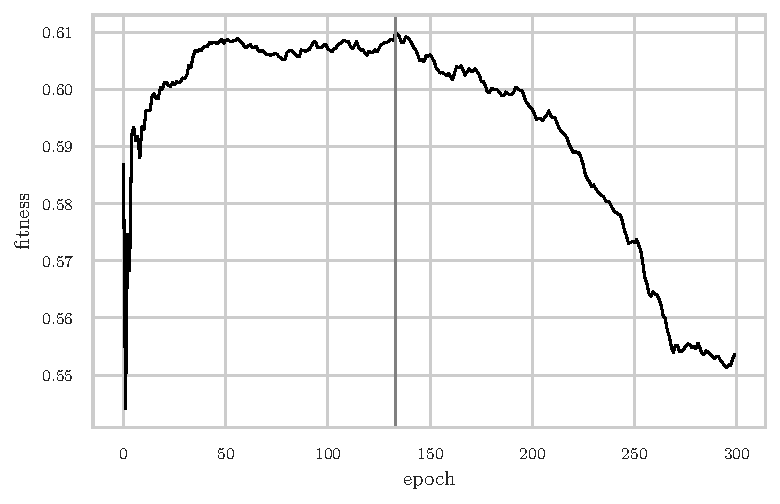
\includegraphics{graphics/model_fitness.pdf}
  \caption[Object detection fitness per epoch.]{Object detection model
    fitness for each epoch calculated as in
    equation~\ref{eq:fitness}. The vertical gray line at 133 marks the
    epoch with the highest fitness.}
  \label{fig:fitness}
\end{figure}

Overall precision and recall per epoch are shown in
figure~\ref{fig:prec-rec}. The values indicate that neither precision
nor recall change materially during training. In fact, precision
starts to decrease from the beginning, while recall experiences a
barely noticeable increase. Taken together with the box and object
loss from figure~\ref{fig:box-obj-loss}, we speculate that the
pre-trained model already generalizes well to plant detection because
one of the categories in the COCO~\cite{lin2015} dataset is
\emph{potted plant}. Any further training solely impacts the
confidence of detection, but does not lead to higher detection
rates. This conclusion is supported by the increasing
\textsf{mAP}@0.5:0.95 until epoch 133.

\begin{figure}
  \centering
  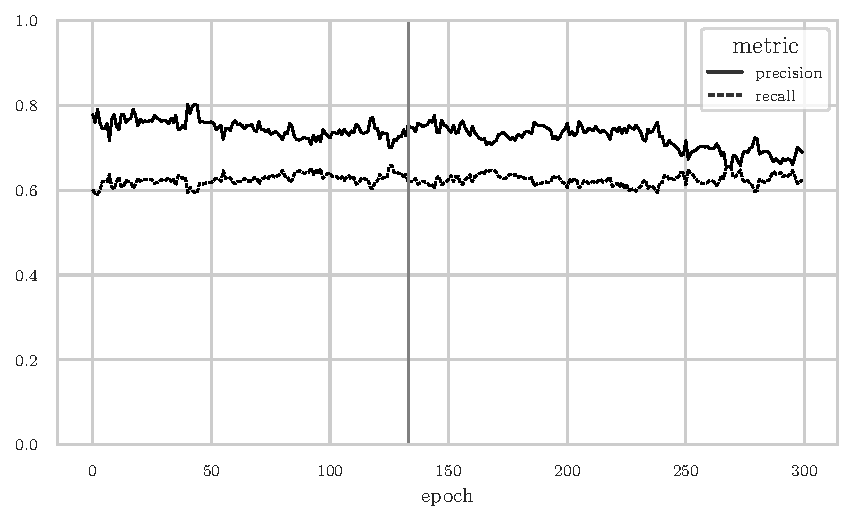
\includegraphics{graphics/precision_recall.pdf}
  \caption[Object detection precision and recall during
  training.]{Overall precision and recall during training for each
    epoch. The vertical gray line at 133 marks the epoch with the
    highest fitness.}
  \label{fig:prec-rec}
\end{figure}

Further culprits for the flat precision and recall values may be found
in bad ground truth data. The labels from the \gls{oid} are sometimes not
fine-grained enough. Images which contain multiple individual—often
overlapping—plants are labeled with one large bounding box instead of
multiple smaller ones. The model recognizes the individual plants and
returns tighter bounding boxes even if that is not what is specified
in the ground truth. Therefore, it is prudent to limit the training
phase to relatively few epochs in order to not penalize the more
accurate detections of the model. The smaller bounding boxes make more
sense considering the fact that the cutout is passed to the classifier
in a later stage. Smaller bounding boxes help the classifier to only
focus on one plant at a time and to not get distracted by multiple
plants in potentially different stages of wilting.

The box loss decreases slightly during training which indicates that
the bounding boxes become tighter around objects of interest. With
increasing training time, however, the object loss increases,
indicating that less and less plants are present in the predicted
bounding boxes. It is likely that overfitting is a cause for the
increasing object loss from epoch 40 onward. Since the best weights as
measured by fitness are found at epoch 133 and the object loss
accelerates from that point, epoch 133 is probably the correct cutoff
before overfitting occurs.

\begin{figure}
  \centering
  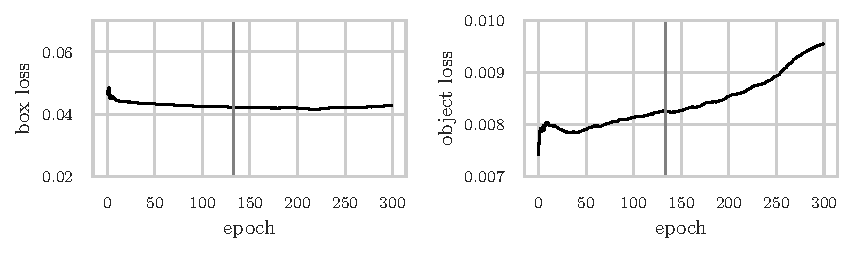
\includegraphics{graphics/val_box_obj_loss.pdf}
  \caption[Object detection box and object loss.]{Box and object loss
    measured against the validation set of 3091 images and 4092 ground
    truth labels. The class loss is omitted because there is only one
    class in the dataset and the loss is therefore always zero.}
  \label{fig:box-obj-loss}
\end{figure}

\subsection{Test Phase}
\label{ssec:yolo-test}

Of the 91479 images around 10\% were used for the test phase. These
images contain a total of 12238 ground truth
labels. Table~\ref{tab:yolo-metrics} shows precision, recall and the
harmonic mean of both (F1-score). The results indicate that the model
errs on the side of sensitivity because recall is higher than
precision. Although some detections are not labeled as plants in the
dataset, if there is a labeled plant in the ground truth data, the
chance is high that it will be detected. This behavior is in line with
how the model's detections are handled in practice. The detections are
drawn on the original image and the user is able to check the bounding
boxes visually. If there are wrong detections, the user can ignore
them and focus on the relevant ones instead. A higher recall will thus
serve the user's needs better than a high precision.

\begin{table}[h]
  \centering
  \begin{tabular}{lrrrr}
    \toprule
    {} &  Precision &    Recall &  F1-score &  Support \\
    \midrule
    Plant        &   0.547571 &  0.737866 &  0.628633 &  12238.0 \\
    \bottomrule
  \end{tabular}
  \caption{Precision, recall and F1-score for the object detection model.}
  \label{tab:yolo-metrics}
\end{table}

Figure~\ref{fig:yolo-ap} shows the \gls{ap} for the \gls{iou}
thresholds of 0.5 and 0.95. Predicted bounding boxes with an \gls{iou}
of less than 0.5 are not taken into account for the precision and
recall values of table~\ref{tab:yolo-metrics}. The lower the detection
threshold, the more plants are detected. Conversely, a higher
detection threshold leaves potential plants undetected. The
precision-recall curves confirm this behavior because the area under
the curve for the threshold of 0.5 is higher than for the threshold of
0.95 ($0.66$ versus $0.41$). These values are combined in COCO's
\cite{lin2015} main evaluation metric which is the \gls{ap} averaged
across the \gls{iou} thresholds from 0.5 to 0.95 in 0.05 steps. This
value is then averaged across all classes and called \gls{map}. The
object detection model achieves a state-of-the-art \gls{map} of 0.5727
for the \emph{Plant} class.

\begin{figure}
  \centering
  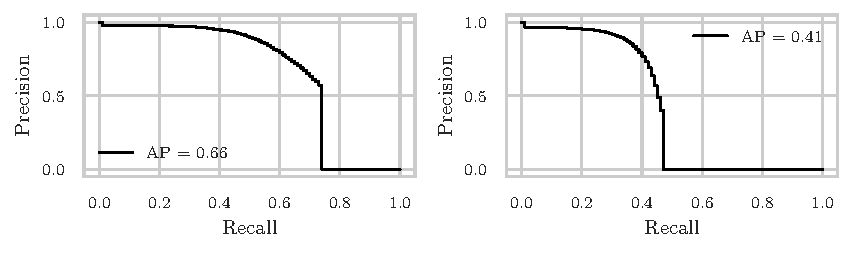
\includegraphics{graphics/APpt5-pt95.pdf}
  \caption[Object detection AP@0.5 and AP@0.95.]{Precision-recall
    curves for \gls{iou} thresholds of 0.5 and 0.95. The \gls{ap} of a
    specific threshold is defined as the area under the
    precision-recall curve of that threshold. The \gls{map} across
    \gls{iou} thresholds from 0.5 to 0.95 in 0.05 steps
    \textsf{mAP}@0.5:0.95 is 0.5727.}
  \label{fig:yolo-ap}
\end{figure}

\subsection{Hyper-parameter Optimization}
\label{ssec:yolo-hyp-opt}

To further improve the object detection performance, we perform
hyper-parameter optimization using a genetic algorithm. Evolution of
the hyper-parameters starts from the initial 30 default values
provided by the authors of YOLO. Of those 30 values, 26 are allowed to
mutate. During each generation, there is an 80\% chance that a
mutation occurs with a variance of 0.04. To determine which generation
should be the parent of the new mutation, all previous generations are
ordered by fitness in decreasing order. At most five top generations
are selected and one of them is chosen at random. Better generations
have a higher chance of being selected as the selection is weighted by
fitness. The parameters of that chosen generation are then mutated
with the aforementioned probability and variance. Each generation is
trained for three epochs and the fitness of the best epoch is
recorded.

In total, we ran 87 iterations of which the 34\textsuperscript{th}
generation provides the best fitness of 0.6076. Due to time
constraints, it was not possible to train each generation for more
epochs or to run more iterations in total. We assume that the
performance of the first few epochs is a reasonable proxy for model
performance overall. The optimized version of the object detection
model is then trained for 70 epochs using the parameters of the
34\textsuperscript{th} generation.

\begin{figure}
  \centering
  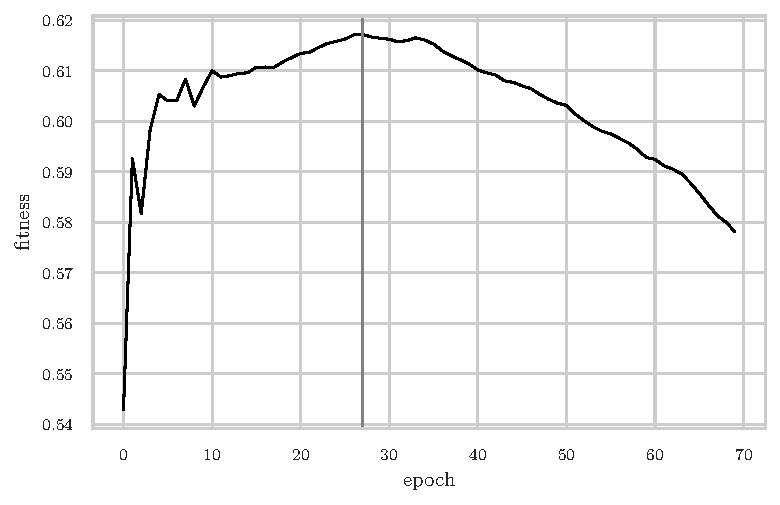
\includegraphics{graphics/model_fitness_final.pdf}
  \caption[Optimized object detection fitness per epoch.]{Object
    detection model fitness for each epoch calculated as in
    equation~\ref{eq:fitness}. The vertical gray line at 27 marks the
    epoch with the highest fitness of 0.6172.}
  \label{fig:hyp-opt-fitness}
\end{figure}

Figure~\ref{fig:hyp-opt-fitness} shows the model's fitness during
training for each epoch. After the highest fitness of 0.6172 at epoch
27, the performance quickly declines and shows that further training
would likely not yield improved results. The model converges to its
highest fitness much earlier than the non-optimized version, which
indicates that the adjusted parameters provide a better starting point
in general. Furthermore, the maximum fitness is 0.74\% higher than in
the non-optimized version.

\begin{figure}
  \centering
  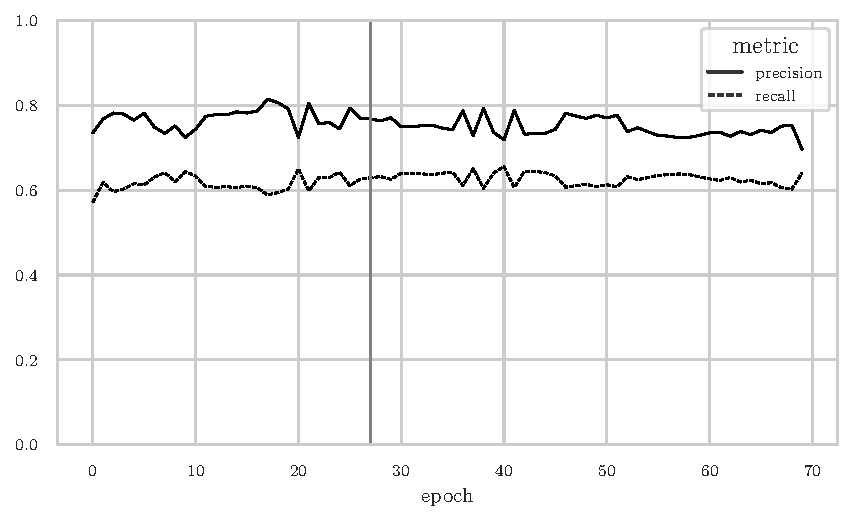
\includegraphics{graphics/precision_recall_final.pdf}
  \caption[Hyper-parameter optimized object detection precision and
  recall during training.]{Overall precision and recall during
    training for each epoch of the optimized model. The vertical gray
    line at 27 marks the epoch with the highest fitness.}
  \label{fig:hyp-opt-prec-rec}
\end{figure}

Figure~\ref{fig:hyp-opt-prec-rec} shows precision and recall for the
optimized model during training. Similarly to the non-optimized model
from figure~\ref{fig:prec-rec}, both metrics do not change materially
during training. Precision is slightly higher than in the
non-optimized version and recall hovers at the same levels.

\begin{figure}
  \centering
  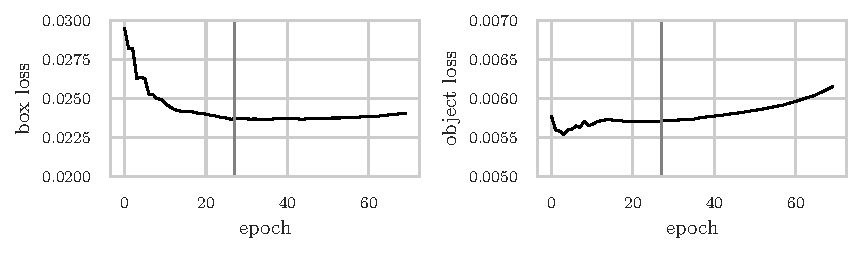
\includegraphics{graphics/val_box_obj_loss_final.pdf}
  \caption[Hyper-parameter optimized object detection box and object
  loss.]{Box and object loss measured against the validation set of
    3091 images and 4092 ground truth labels. The class loss is
    omitted because there is only one class in the dataset and the
    loss is therefore always zero.}
  \label{fig:hyp-opt-box-obj-loss}
\end{figure}

The box and object loss during training is pictured in
figure~\ref{fig:hyp-opt-box-obj-loss}. Both losses start from a lower
level which suggests that the initial optimized parameters allow the
model to converge quicker. The object loss exhibits a similar slope to
the non-optimized model in figure~\ref{fig:box-obj-loss}. The vertical
gray line again marks epoch 27 with the highest fitness. The box loss
reaches its lower limit at that point and the object loss starts to
increase again after epoch 27.

\begin{table}[h]
  \centering
  \begin{tabular}{lrrrr}
    \toprule
    {} &  Precision &    Recall &  F1-score &  Support \\
    \midrule
    Plant        &   0.633358 &  0.702811 &  0.666279 &  12238.0 \\
    \bottomrule
  \end{tabular}
  \caption{Precision, recall and F1-score for the optimized object
    detection model.}
  \label{tab:yolo-metrics-hyp}
\end{table}

Turning to the evaluation of the optimized model on the test dataset,
table~\ref{tab:yolo-metrics-hyp} shows precision, recall and the
F1-score for the optimized model. Comparing these metrics with the
non-optimized version from table~\ref{tab:yolo-metrics}, precision is
significantly higher by more than 8.5\%. Recall, however, is 3.5\%
lower. The F1-score is higher by more than 3.7\% which indicates that
the optimized model is better overall despite the lower recall. We
feel that the lower recall value is a suitable trade off for the
substantially higher precision considering that the non-optimized
model's precision is quite low at 0.55.

The precision-recall curves in figure~\ref{fig:yolo-ap-hyp} for the
optimized model show that the model draws looser bounding boxes than
the optimized model. The \gls{ap} for both \gls{iou} thresholds of 0.5
and 0.95 is lower indicating worse performance. It is likely that more
iterations during evolution would help increase the \gls{ap} values as
well. Even though the precision and recall values from
table~\ref{tab:yolo-metrics-hyp} are better, the \textsf{mAP}@0.5:0.95
is lower by 1.8\%.

\begin{figure}
  \centering
  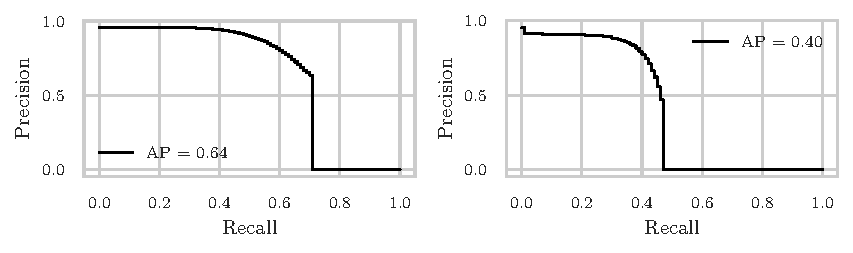
\includegraphics{graphics/APpt5-pt95-final.pdf}
  \caption[Hyper-parameter optimized object detection AP@0.5 and
  AP@0.95.]{Precision-recall curves for \gls{iou} thresholds of 0.5
    and 0.95. The \gls{ap} of a specific threshold is defined as the
    area under the precision-recall curve of that threshold. The
    \gls{map} across \gls{iou} thresholds from 0.5 to 0.95 in 0.05
    steps \textsf{mAP}@0.5:0.95 is 0.5546.}
  \label{fig:yolo-ap-hyp}
\end{figure}

\section{Classification}
\label{sec:classifier-eval}

The classifier receives cutouts from the object detection model and
determines whether the image shows a stressed plant or not. To achieve
this goal, we trained a \gls{resnet} \cite{he2016} on a dataset of 452
images of healthy and 452 stressed plants. We chose the \gls{resnet}
architecture due to its popularity and ease of implementation as well
as its consistently high performance on various classification
tasks. While its classification speed in comparison with networks
optimized for mobile and edge devices (e.g. MobileNet) is
significantly lower, the deeper structure and the additional
parameters are necessary for the fairly complex task at
hand. Furthermore, the generous time budget for object detection
\emph{and} classification allows for more accurate results at the
expense of speed. The architecture allows for multiple different
structures, depending on the amount of layers. The smallest one has 18
and the largest 152 layers with 34, 50 and 101 in-between. The larger
networks have better accuracy in general, but come with trade-offs
regarding training and inference time as well as required space. The
50 layer architecture (\gls{resnet}50) is adequate for our use case.

\subsection{Training Phase}
\label{ssec:classifier-training}

The dataset was split 85/15 into training and validation sets. The
images in the training set were augmented with a random crop to arrive
at the expected image dimensions of 224 pixels. Additionally, the
training images were modified with a random horizontal flip to
increase the variation in the set and to train a rotation invariant
classifier. All images, regardless of their membership in the training
or validation set, were normalized with the mean and standard
deviation of the ImageNet~\cite{deng2009} dataset, which the original
\gls{resnet} model was pre-trained with. Training was done for 50
epochs and the best-performing model as measured by validation
accuracy was selected as the final version.

Figure~\ref{fig:classifier-training-metrics} shows accuracy and loss
on the training and validation sets. There is a clear upwards trend
until epoch 20 when validation accuracy and loss stabilize at around
0.84 and 0.3, respectively. The quick convergence and resistance to
overfitting can be attributed to the model already having robust
feature extraction capabilities.

\begin{figure}
  \centering
  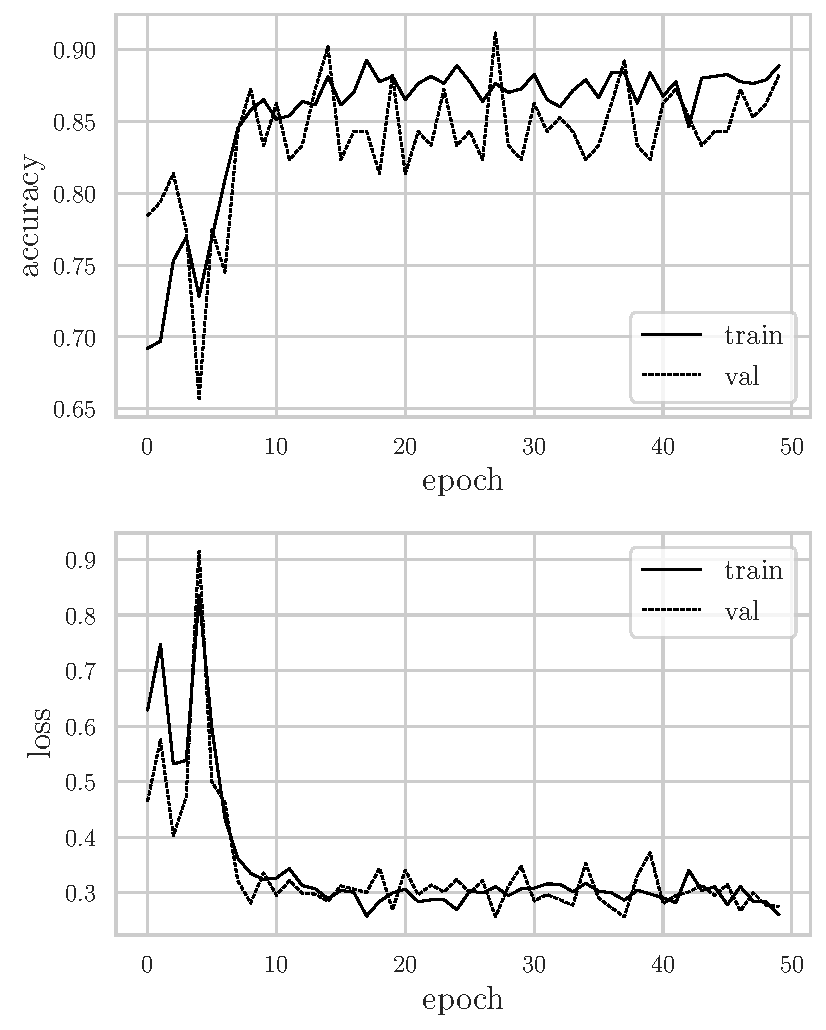
\includegraphics{graphics/classifier-metrics.pdf}
  \caption[Classifier accuracy and loss during training.]{Accuracy and
    loss during training of the classifier. The model converges
    quickly, but additional epochs do not cause validation loss to
    increase, which would indicate overfitting. The maximum validation
    accuracy of 0.9118 is achieved at epoch 27.}
  \label{fig:classifier-training-metrics}
\end{figure}

\subsection{Hyper-parameter Optimization}
\label{ssec:classifier-hyp-opt}

In order to improve the aforementioned accuracy values, we perform
hyper-parameter optimization across a wide range of
parameters. Table~\ref{tab:classifier-hyps} lists the hyper-parameters
and their possible values. Since the number of all combinations of
values is 11520 and each combination is trained for 10 epochs with a
training time of approximately six minutes per combination, exhausting
the search space would take 48 days. Due to time limitations, we have
chosen to not search exhaustively but to pick random combinations
instead. Random search works surprisingly well---especially compared to
grid search---in a number of domains, one of which is hyper-parameter
optimization~\cite{bergstra2012}.

\begin{table}[h]
  \centering
  \begin{tabular}{lr}
    \toprule
    Parameter &  Values \\
    \midrule
    optimizer &	adam, sgd \\
    batch size & 4, 8, 16, 32, 64 \\
    learning rate & 0.0001, 0.0003, 0.001, 0.003, 0.01, 0.1 \\
    step size & 2, 3, 5, 7 \\
    gamma & 0.1, 0.5 \\
    beta one & 0.9, 0.99 \\
    beta two & 0.5, 0.9, 0.99, 0.999 \\
    eps & 0.00000001, 0.1, 1 \\
    \bottomrule
  \end{tabular}
  \caption{Hyper-parameters and their possible values during
    optimization.}
  \label{tab:classifier-hyps}
\end{table}

The random search was run for 138 iterations which equates to a 75\%
probability that the best solution lies within 1\% of the theoretical
maximum~\eqref{eq:opt-prob}. Figure~\ref{fig:classifier-hyp-results}
shows three of the eight parameters and their impact on a high
F1-score. \gls{sgd} has less variation in its results than
Adam~\cite{kingma2017} and manages to provide eight out of the ten
best results. The number of epochs to train for was chosen based on
the observation that almost all configurations converge well before
reaching the tenth epoch. The assumption that a training run with ten
epochs provides a good proxy for final performance is supported by the
quick convergence of validation accuracy and loss in
figure~\ref{fig:classifier-training-metrics}.

\begin{equation}\label{eq:opt-prob}
  1 - (1 - 0.01)^{138} \approx 0.75
\end{equation}

\begin{figure}
  \centering
  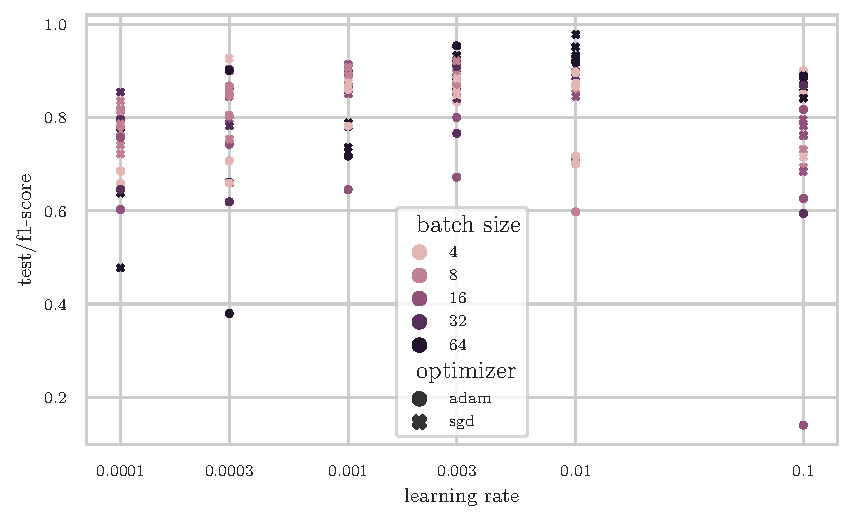
\includegraphics{graphics/classifier-hyp-metrics.pdf}
  \caption[Classifier hyper-parameter optimization results.]{This
    figure shows three of the eight hyper-parameters and their
    performance measured by the F1-score during 138
    trials. Differently colored markers show the batch size with
    darker colors representing a larger batch size. The type of marker
    (circle or cross) shows which optimizer was used. The x-axis shows
    the learning rate on a logarithmic scale. In general, a learning
    rate between 0.003 and 0.01 results in more robust and better
    F1-scores. Larger batch sizes more often lead to better
    performance as well. As for the type of optimizer, \gls{sgd}
    produced the best iteration with an F1-score of 0.9783. Adam tends
    to require more customization of its parameters than \gls{sgd} to
    achieve good results.}
  \label{fig:classifier-hyp-results}
\end{figure}

Table~\ref{tab:classifier-final-hyps} lists the final hyper-parameters
which were chosen to train the improved model. In order to confirm
that the model does not suffer from overfitting or is a product of
chance due to a coincidentally advantageous train/test split, we
perform stratified $10$-fold cross validation on the dataset. Each
fold contains 90\% training and 10\% test data and was trained for 25
epochs. Figure~\ref{fig:classifier-hyp-roc} shows the performance of
the epoch with the highest F1-score of each fold as measured against
the test split. The mean \gls{roc} curve provides a robust metric for
a classifier's performance because it averages out the variability of
the evaluation. Each fold manages to achieve at least an \gls{auc} of
0.94, while the best fold reaches 0.98. The mean \gls{roc} has an
\gls{auc} of 0.96 with a standard deviation of 0.02. These results
indicate that the model is accurately predicting the correct class and
is robust against variations in the training set.

\begin{table}
  \centering
  \begin{tabular}{cccc}
    \toprule
    Optimizer &  Batch Size & Learning Rate & Step Size \\
    \midrule
    \gls{sgd} & 64 & 0.01 & 5\\
    \bottomrule
  \end{tabular}
  \caption[Hyper-parameters for the optimized classifier.]{Chosen
    hyper-parameters for the final, improved model. The difference to
    the parameters listed in Table~\ref{tab:classifier-hyps} comes as
    a result of choosing \gls{sgd} over Adam. The missing four
    parameters are only required for Adam and not \gls{sgd}.}
  \label{tab:classifier-final-hyps}
\end{table}

\begin{figure}
  \centering
  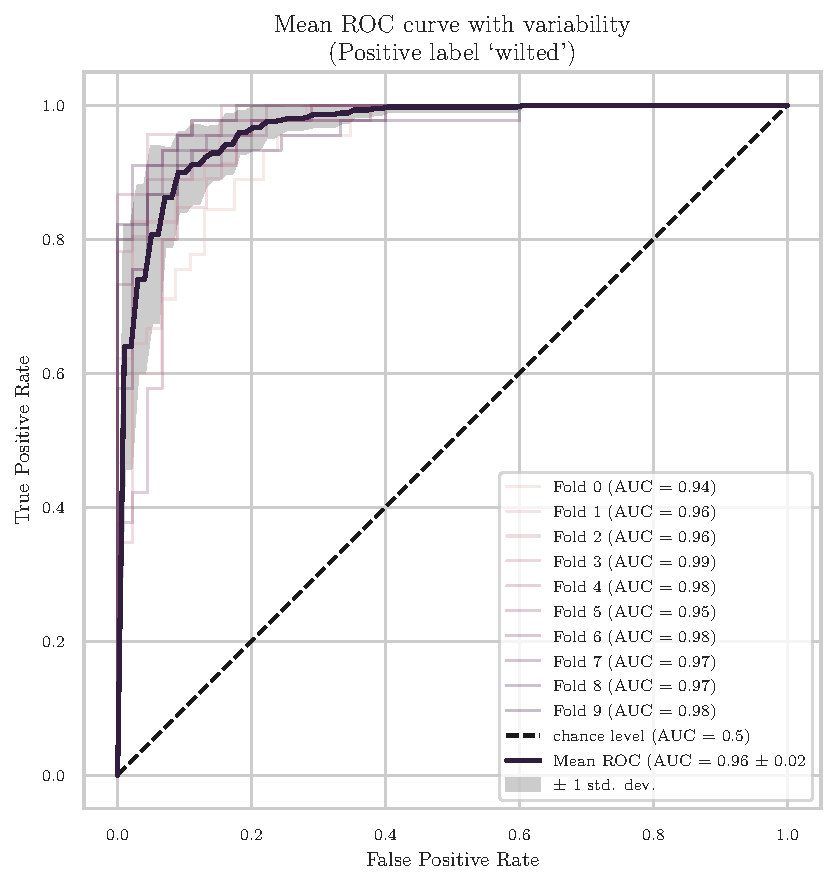
\includegraphics{graphics/classifier-hyp-folds-roc.pdf}
  \caption[Mean \gls{roc} and variability of hyper-parameter-optimized
  model.]{This plot shows the \gls{roc} curve for the epoch with the
    highest F1-score of each fold as well as the \gls{auc}. To get a
    less variable performance metric of the classifier, the mean
    \gls{roc} curve is shown as a thick line and the variability is
    shown in gray. The overall mean \gls{auc} is 0.96 with a standard
    deviation of 0.02. The best-performing fold reaches an \gls{auc}
    of 0.99 and the worst an \gls{auc} of 0.94. The black dashed line
    indicates the performance of a classifier which picks classes at
    random ($\mathrm{\gls{auc}} = 0.5$). The shapes of the \gls{roc}
    curves show that the classifier performs well and is robust
    against variations in the training set.}
  \label{fig:classifier-hyp-roc}
\end{figure}

The classifier shows good performance so far, but care has to be taken
to not overfit the model to the training set. Comparing the F1-score
during training with the F1-score during testing gives insight into
when the model tries to increase its performance during training at
the expense of generalizability. Figure~\ref{fig:classifier-hyp-folds}
shows the F1-scores of each epoch and fold. The classifier converges
quickly to 1 for the training set at which point it experiences a
slight drop in generalizability. Training the model for at most five
epochs is sufficient because there are generally no improvements
afterwards. The best-performing epoch for each fold is between the
second and fourth epoch which is just before the model achieves an
F1-score of 1 on the training set.

\begin{figure}
  \centering
  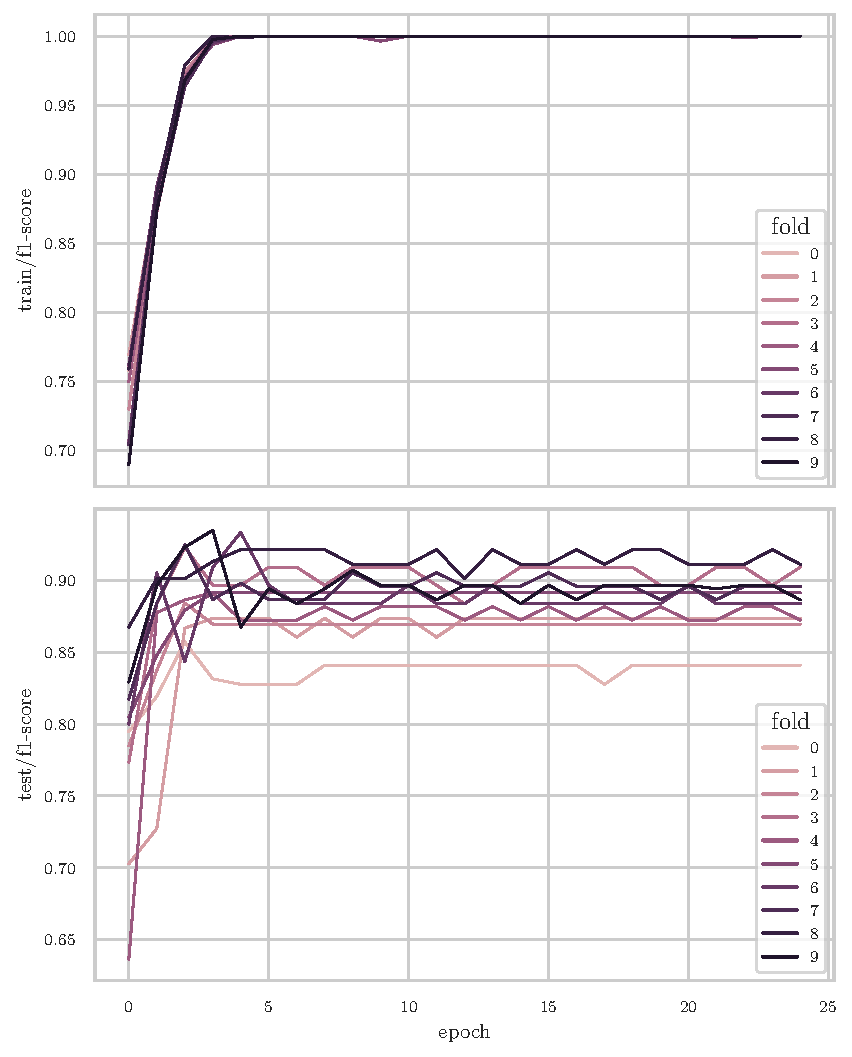
\includegraphics[width=.9\textwidth]{graphics/classifier-hyp-folds-f1.pdf}
  \caption[F1-score of stratified $10$-fold cross validation.]{These
    plots show the F1-score during training as well as testing for
    each of the folds. The classifier converges to 1 by the third
    epoch during the training phase, which might indicate
    overfitting. However, the performance during testing increases
    until epoch three in most cases and then stabilizes at
    approximately 2-3\% lower than the best epoch. We believe that the
    third, or in some cases fourth, epoch is detrimental to
    performance and results in overfitting, because the model achieves
    an F1-score of 1 for the training set, but that gain does not
    transfer to the test set. Early stopping during training
    alleviates this problem.}
  \label{fig:classifier-hyp-folds}
\end{figure}


\subsection{Class Activation Maps}
\label{ssec:classifier-cam}

Neural networks are notorious for their black-box behavior, where it
is possible to observe the inputs and the corresponding outputs, but
the stage in-between stays hidden from view. Models are continuously
developed and deployed to aid in human decision-making and sometimes
supplant it. It is, therefore, crucial to obtain some amount of
interpretability of what the model does \emph{inside} to be able to
explain why a decision was made in a certain way. The research field
of \gls{xai} gained significance during the last few years because of
the development of new methods to peek inside these black boxes.

One such method, \gls{cam}~\cite{zhou2015}, is a popular tool to
produce visual explanations for decisions made by
\glspl{cnn}. Convolutional layers essentially function as object
detectors as long as no fully-connected layers perform the
classification. This ability to localize regions of interest, which
play a significant role in the type of class the model predicts, can
be retained until the last layer and used to generate activation maps
for the predictions.

A more recent approach to generating a \gls{cam} via gradients is
proposed by~\textcite{selvaraju2020}. Their \gls{grad-cam} approach
works by computing the gradient of the feature maps of the last
convolutional layer with respect to the specified class. The last
layer is chosen because the authors find that ``[…]  Grad-CAM maps
become progressively worse as we move to earlier convolutional layers
as they have smaller receptive fields and only focus on less semantic
local features.''~\cite[p.5]{selvaraju2020}

Turning to our classifier, figure~\ref{fig:classifier-cam} shows the
\glspl{cam} for \emph{healthy} and \emph{stressed}. While the regions
of interest for the \emph{healthy} class lie on the healthy plant, the
\emph{stressed} plant is barely considered and mostly rendered as
background information (blue). Conversely, when asked to explain the
inputs to the \emph{stressed} classification, the regions of interest
predominantly stay on the thirsty as opposed to the healthy plant. In
fact, the large hanging leaves play a significant role in determining
the class the image belongs to. This is an additional data point
confirming that the model focuses on the semantically meaningful parts
of the image during classification.

\begin{figure}
  \centering
  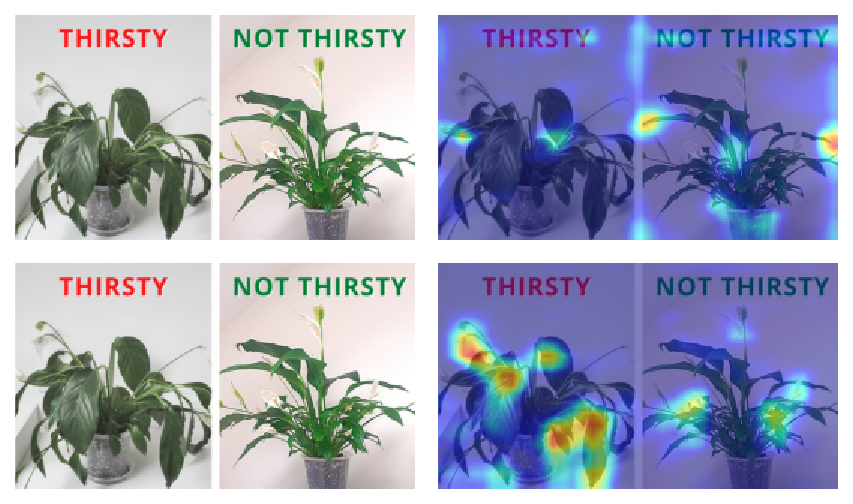
\includegraphics{graphics/classifier-cam.pdf}
  \caption[Classifier \glspl{cam}.]{The top left image shows the
    original image of the same plant in a stressed (left) and healthy
    (right) state. In the top right image, the \gls{cam} for the class
    \emph{healthy} is laid over the original image. The classifier
    draws its conclusion mainly from the healthy plant, which is
    indicated by the red hot spots around the tips of the plant. The
    bottom right image shows the \gls{cam} for the \emph{stressed}
    class. The classifier focuses on the hanging leaves of the thirsty
    plant. The image was classified as \emph{stressed} with a
    confidence of 70\%.}
  \label{fig:classifier-cam}
\end{figure}


\section{Aggregate Model}
\label{sec:aggregate-model}

In this section we turn to the evaluation of the aggregate model. We
have confirmed the performance of the constituent models: the object
detection and the classification model. It remains to evaluate the
complete pipeline from gathering detections of potential plants in an
image and forwarding them to the classifier to obtaining the results
as either healthy or stressed with their associated confidence scores.

The test set contains 640 images which were obtained from a google
search using the terms \emph{thirsty plant}, \emph{wilted plant} and
\emph{stressed plant}. Images which clearly show one or multiple
plants with some amount of visible stress were added to the
dataset. Care was taken to include plants with various degrees of
stress and in various locations and lighting conditions. The search
not only provided images of stressed plants, but also of healthy
plants due to articles, which describe how to care for plants, having
a banner image of healthy plants. The dataset is biased towards potted
plants which are commonly put on display in western
households. Furthermore, many plants, such as succulents, are sought
after for home environments because of their ease of maintenance. Due
to their inclusion in the dataset and how they exhibit water stress,
the test set nevertheless contains a wide variety of scenarios.

After collecting the images, the aggregate model was run on them to
obtain initial bounding boxes and classifications for ground truth
labeling. Letting the model do the work beforehand and then correcting
the labels allowed to include more images in the test set because they
could be labeled more easily. Additionally, going over the detections
and classifications provided a comprehensive view on how the models
work and what their weaknesses and strengths are. After the labels
have been corrected, the ground truth of the test set contains 766
bounding boxes of healthy plants and 494 of stressed plants.

\subsection{Non-optimized Model}
\label{ssec:model-non-optimized}

\begin{table}
  \centering
  \begin{tabular}{lrrrr}
    \toprule
    {} &  precision &  recall &  f1-score &  support \\
    \midrule
    Healthy      &      0.665 &   0.554 &     0.604 &    766 \\
    Stressed     &      0.639 &   0.502 &     0.562 &    494 \\
    micro avg    &      0.655 &   0.533 &     0.588 &   1260 \\
    macro avg    &      0.652 &   0.528 &     0.583 &   1260 \\
    weighted avg &      0.655 &   0.533 &     0.588 &   1260 \\
    \bottomrule
  \end{tabular}
  \caption{Precision, recall and F1-score for the aggregate model.}
  \label{tab:model-metrics}
\end{table}

Table~\ref{tab:model-metrics} shows precision, recall and the F1-score
for both classes \emph{Healthy} and \emph{Stressed}. Precision is
higher than recall for both classes and the F1-score is at
0.59. Unfortunately, these values do not take the accuracy of bounding
boxes into account and thus have only limited expressive power.

Figure~\ref{fig:aggregate-ap} shows the precision and recall curves
for both classes at different \gls{iou} thresholds. The left plot
shows the \gls{ap} for each class at the threshold of 0.5 and the
right one at 0.95. The \gls{map} is 0.3581 and calculated across all
classes as the median of the \gls{iou} thresholds from 0.5 to 0.95 in
0.05 steps. The cliffs at around 0.6 (left) and 0.3 (right) happen at
a detection threshold of 0.5. The classifier's last layer is a softmax
layer which necessarily transforms the input into a probability of
showing either a healthy or stressed plant. If the probability of an
image showing a healthy plant is below 0.5, it is no longer classified
as healthy but as stressed. The threshold for discriminating the two
classes lies at the 0.5 value and is therefore the cutoff for either
class.

\begin{figure}
  \centering
  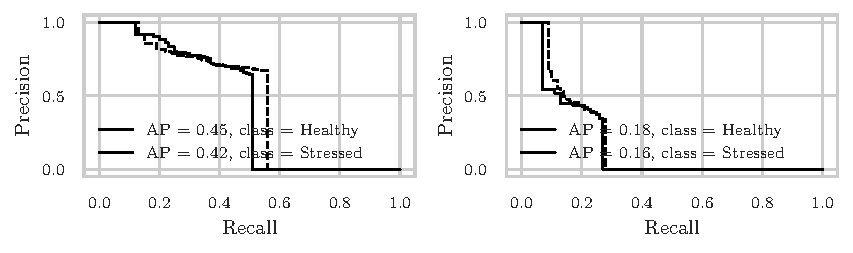
\includegraphics{graphics/APmodel-model-optimized-relabeled.pdf}
  \caption[Aggregate model AP@0.5 and AP@0.95.]{Precision-recall
    curves for \gls{iou} thresholds of 0.5 and 0.95. The \gls{ap} of a
    specific threshold is defined as the area under the
    precision-recall curve of that threshold. The \gls{map} across
    \gls{iou} thresholds from 0.5 to 0.95 in 0.05 steps
    \textsf{mAP}@0.5:0.95 is 0.3581.}
  \label{fig:aggregate-ap}
\end{figure}

\subsection{Optimized Model}
\label{ssec:model-optimized}

So far the metrics shown in table~\ref{tab:model-metrics} are obtained
with the non-optimized versions of both the object detection and
classification model. Hyper-parameter optimization of the classifier
led to significant model improvements, while the object detector has
improved precision but lower recall and slightly lower \gls{map}
values. To evaluate the final aggregate model which consists of the
individual optimized models, we run the same test described in
section~\ref{sec:aggregate-model}.

\begin{table}
  \centering
  \begin{tabular}{lrrrr}
    \toprule
    {} &  precision &  recall &  f1-score &  support \\
    \midrule
    Healthy      &      0.711 &   0.555 &     0.623 &    766 \\
    Stressed     &      0.570 &   0.623 &     0.596 &    494 \\
    micro avg    &      0.644 &   0.582 &     0.611 &   1260 \\
    macro avg    &      0.641 &   0.589 &     0.609 &   1260 \\
    weighted avg &      0.656 &   0.582 &     0.612 &   1260 \\
    \bottomrule
  \end{tabular}
  \caption{Precision, recall and F1-score for the optimized aggregate
    model.}
  \label{tab:model-metrics-hyp}
\end{table}

Table~\ref{tab:model-metrics-hyp} shows precision, recall and F1-score
for the optimized model on the same test dataset of 640 images. All of
the metrics are better for the optimized model. In particular,
precision for the healthy class could be improved significantly while
recall remains at the same level. This results in a better F1-score
for the healthy class. Precision for the stressed class is lower with
the optimized model, but recall is significantly higher (0.502
vs. 0.623). The higher recall results in a 3\% gain for the F1-score
in the stressed class. Overall, precision is the same but recall has
improved significantly, which also results in a noticeable improvement
for the average F1-score across both classes.

\begin{figure}
  \centering
  \includegraphics{graphics/APModel-model-original-relabeled.pdf}
  \caption[Optimized aggregate model AP@0.5 and
  AP@0.95.]{Precision-recall curves for \gls{iou} thresholds of 0.5
    and 0.95. The \gls{ap} of a specific threshold is defined as the
    area under the precision-recall curve of that threshold. The
    \gls{map} across \gls{iou} thresholds from 0.5 to 0.95 in 0.05
    steps \textsf{mAP}@0.5:0.95 is 0.3838.}
  \label{fig:aggregate-ap-hyp}
\end{figure}

Figure~\ref{fig:aggregate-ap-hyp} confirms the performance increase of
the optimized model established in
table~\ref{tab:model-metrics-hyp}. The \textsf{mAP}@0.5 is higher for
both classes, indicating that the model better detects plants in
general. The \textsf{mAP}@0.95 is slightly lower for the healthy
class, which means that the confidence for the healthy class is
slightly lower compared to the non-optimized model. The result is that
more plants are correctly detected and classified overall, but the
confidence scores tend to be lower with the optimized model. The
\textsf{mAP}@0.5:0.95 could be improved by about 0.025.

\backmatter

% Use an optional list of figures.
\listoffigures % Starred version, i.e., \listoffigures*, removes the toc entry.

% Use an optional list of tables.
\cleardoublepage % Start list of tables on the next empty right hand page.
\listoftables % Starred version, i.e., \listoftables*, removes the toc entry.

% Use an optional list of algorithms.
\listofalgorithms
\addcontentsline{toc}{chapter}{List of Algorithms}

% Add an index.
\printindex

% Add a glossary.
\printglossaries

% Add a bibliography.
%\bibliographystyle{alpha}
\printbibliography

\end{document}
%%% Local Variables:
%%% mode: latex
%%% TeX-master: t
%%% TeX-master: t
%%% TeX-master: t
%%% TeX-master: "thesis"
%%% End:
